\documentclass[12pt]{article}

% House style preamble
\input{.house-style/preamble.tex}
\usepackage{float}
\usepackage{tikz}
\usetikzlibrary{arrows.meta}
% Figure idiom, greyscale-safe because Synthese prints mono: no colour carries a
% distinction, and every contrast is line style, position, or label.
\tikzset{
  ttpbox/.style={draw, rounded corners=2pt, align=center, inner sep=4pt,
                 minimum height=7.5mm, font=\small},
  ttpar/.style={-{Stealth[length=2mm]}, thick},
  ttpblocked/.style={-{Stealth[length=2mm]}, thick, dashed, draw=black},
  ttplab/.style={font=\scriptsize\itshape, inner sep=2pt},
}

% Update PDF metadata
\hypersetup{
  pdftitle={Grounding Without Corrective Control: Truth-Tracking Profiles for Large Language Models},
  pdfkeywords={large language models; grounding; answerability; corrective control; projectibility; truth-tracking; philosophy of AI}
}

% The project's preamble snapshot predates \aidisclosure (added centrally 2026-07-16).
% Defined here rather than by refreshing the snapshot, which carries guarded local font
% paths this build depends on. Drop this block when the snapshot is refreshed.

\providecommand{\aidisclosure}[1]{%
  \par\medskip
  \noindent{\small\textsc{AI use.}\enspace The large language models #1 served as
  drafting and editing aids throughout the preparation of this paper. I'm
  responsible for all theoretical claims, arguments, errors, and interpretive
  choices.\par}%
  \medskip
}

\title{Grounding Without Corrective Control:\\ Truth-Tracking Profiles for Large Language Models}
\author{Brett Reynolds \orcidlink{0000-0003-0073-7195}%
\thanks{Contact: \href{mailto:brett.reynolds@humber.ca}{brett.reynolds@humber.ca}}\\
Humber Polytechnic \& University of Toronto}
\date{\today}

\begin{document}
\maketitle

\begin{abstract}
Recent work makes a strong case that at least some large language model representations
have content or reference. That leaves a different question open. Grounding can secure
content, reference, or correctness conditions without supplying the live, sufficiently
independent routes through which a discrepancy with the target is detected and made to
alter production, uptake, withdrawal, or later behaviour. Call the weaker relation
answerability and the stronger one corrective control. This paper analyses both through a
profile: a pattern of participation in routes that supply target contact, integrate
representations, handle discrepancies, and register practical success or failure.
Answerability comes in degrees; corrective control is the case where answerability
includes both detection and an effective route to repair.

Language models provide the pressure case, with the text-only profile taken as a limiting
position rather than a description of a product. Text-trained arrangements inherit dense textual
traces of testimony, local coherence, and corrections already made in the source practices.
That inheritance gives them derivative answerability. Their weak participation in
perception, measurement, intervention, and practical correction leaves them without
corrective control wherever the relevant target isn't reachable through a live checking route.
The result is a familiar failure signature: fluent, coherent outputs that hold up until a
task needs a live, independently informative route to the facts. Self-consistency, retrieval, tools, code
execution, multimodal input, and feedback from human preference judgements or action
outcomes should help only where they supply the route a task requires. Their benefits should
interact with task requirements rather than yield a general gain. A crossed design, varying
route availability against task requirement, can test that prediction. Surface improvement
and truth-tracking improvement can come apart.
\end{abstract}

\noindent\textbf{Keywords:} large language models; grounding; answerability; corrective
control; projectibility; truth-tracking; philosophy of AI

\aidisclosure{Anthropic Claude Opus 4.8, Fable 5, and Opus 5; and OpenAI Codex using
GPT-5.5}

\section{Introduction: from grounding to corrective control}\label{sec:intro}

Do the representations inside large language models (LLMs) connect to the world? The
question is often put as a yes/no. \textcite{bender2020} say no: a system trained on
form alone, like an octopus eavesdropping on telegraph traffic, learns the statistics
of language apart from what language is about. Others reply that such systems
meet at least some conditions on reference, or that sensory grounding can be optional
for thought in the first place
\citep{coelho_mollo_milliere_2026_vector_grounding_problem,chalmers_2023_thought_sensory_grounding_llms}.

But that opposition only starts the inquiry. The debate descends from the symbol-grounding
problem
\citep{harnad_1990_symbol_grounding_problem}: how can symbols, or symbol-like states,
get meaning independent of the interpretations supplied by users? For LLMs, recent work
has already pluralized the issue. \textcite{pavlick_2023_symbols_and_grounding_llms}
treats grounding as a family of questions about symbols and use;
\textcite{coelho_mollo_milliere_2026_vector_grounding_problem} distinguish kinds of
grounding; and \textcite{chalmers_2023_thought_sensory_grounding_llms} separates sensory
grounding from thought.

The recent literature has been closing the sceptical routes one at a time, and closing
them on the side of content. On reference, natural histories of a model's inputs can
secure it \citep{mandelkern_linzen_2024_do_language_models_words_refer}, while intentions
are the wrong place to look \citep{pepp_2025_reference_without_intentions_llms}. On
linguistic competence and meaning, the argument from communicative intention fails at
both premises \citep{attah_2025_do_language_models_lack_communicative_intentions}, and
linguistic metasemantics delivers meaning where mental metasemantics doesn't
\citep{grindrod_2024_large_language_models_linguistic_intentionality}. At the level of the
proposed target, meaning can be grounded in a corpus rather than in the world
\citep{havlik_2024_meaning_understanding_llms_synthese}.
\textcite{ruyant_2026_what_do_llms_represent} reaches the further conclusion that what such
systems represent is a class of appropriate linguistic production rather than the world
at all.

I contest none of those claims, and the argument doesn't require their authors to be
mistaken. Some discuss misrepresentation, error, and repair.\footnote{%
\textcite{coelho_mollo_milliere_2026_vector_grounding_problem} build
the possibility of misrepresentation into their account, and
\textcite{attah_2025_do_language_models_lack_communicative_intentions}
discusses conversational repair. Neither supplies an account of the arrangement-level routes at
issue here, which is the point, and neither is committed to denying that such routes
matter.} What none of it supplies is an account of the live, task-indexed routes through
which a fresh discrepancy becomes detectable and revision-producing. Establishing content
and establishing corrective control are different achievements, and the second doesn't
follow from the first.

Pluralizing grounding still leaves open which dimensions explain truth-relevant success
and failure across arrangements. Truth-tracking success depends on distinct
\term{stabilizers}\footnote{I use \term{stabilizer} for an epistemic route through
which a representation becomes answerable to a declared target. Some stabilizers supply
target contact; others integrate or correct representations already linked to the target. In
\posscite{grindrod_2024_large_language_models_linguistic_intentionality} reading of
Millikan, a \term{stabilizing function} is instead conventional and inter-agent: it sits
between speaker and hearer. It explains why a linguistic device keeps being reproduced,
and he puts the notion to work on language models. A device can have a robust stabilizing
function in Millikan's sense while participating only derivatively in the stabilizers in
mine. That's arguably the text-only case.} that ordinarily operate together: perception,
testimony,
coherence, measurement, intervention, error-correction, and practical
success. An arrangement can take part in some of these and sit out others. The label alone
implies neither effective maintenance nor corrective control.

I argue that these stabilizers form a \term{profile}, and that claims about an
arrangement's profile warrant bounded projections about the successes picked out by the
predicate \mention{true}. The \term{bearer} of the profile and corrective-control
predicates is the target- and task-indexed arrangement that
produces the output. The same model enters different arrangements when a task is answered
from text alone, with retrieved records, through a sensor, or under a checker. The output
itself has no information or correction routes. Taking the surrounding practice without
limit would confer the epistemic credit of human science on every deployment.

A profile, in this sense, isn't a
checklist of individually necessary conditions. It's a pattern of routes whose presence,
absence, and coupling let us project how an arrangement will do in nearby cases
\citep{Goodman1955,khalidi2013}.

LLMs matter because they separate routes that human epistemic life normally bundles
together. The separation is clearest in the limiting case of an arrangement whose contact with
the world remains mediated mainly by previously produced human text rather than live
retrieval, perceptual inputs, execution results, or action outcomes. That case supplies a
baseline, not a description of every LLM arrangement. Against it, retrieval, tools, code execution,
multimodal input, and action-guided feedback make the profile less inheritance-heavy by
adding routes. The question is which route each adds and where the resulting improvement
should transfer.

Each intervention should help only where it supplies the missing route. Self-consistency
should help most where the missing support is coherence; retrieval should help most where
the missing support is record access.
Feedback based on human preference judgements should improve conversational fit before it
improves answerability, the relation that lets discrepancies bear on what an arrangement produces.
Multimodal input should help some perceptual tasks before it helps calibrated measurement.
This profile earns its keep only if these contrasts explain LLM behaviour better than a
single verdict about grounding.

These contrasts concern epistemic architecture rather than the nature of truth.
Correspondence, coherence, pragmatism, reliabilism, and social epistemology each identify a
relation or process that can make representations answerable. Deflationism leaves those
explanatory questions open while denying that truth itself requires a substantive
reduction. This profile asks how these relations and processes combine within an
arrangement and what follows when one is missing. It's a framework for comparison, not a
reconciliation of the underlying theories.

This paper makes three contributions to that architectural project. First, it isolates the
live, task-indexed routes by which a fresh discrepancy reaches production as an explanandum
in their own right rather than a corollary of content. A positive grounding verdict can
settle what a system's representations mean or refer to without licensing an inference
about which fresh errors a deployed arrangement can catch.

Second, it identifies five features that govern whether a fresh discrepancy can reach
production and alter the output in the right direction: target access, detectability,
checking-route independence, attribution, and effective uptake. These features make
answerability a matter of degree, distinguish corrective control as the stronger
architecture, and separate the capacity to correct from its realized effectiveness.

Third, it turns the architecture into a prediction this account can lose. Interventions
supply particular routes, so their benefits should depend on which route a task requires.
The expected result is an interaction between intervention and task rather than a general
gain; indiscriminate transfer would count against the carving. The stronger test is
transport: features characterized in advance should predict new combinations of routes,
tasks, and perturbations without conceptual refitting.

Sections~\ref{sec:target}--\ref{sec:projectibility} define the target, organize the
stabilizers, and state the projections this profile licenses.
Sections~\ref{sec:adjudication} and~\ref{sec:objections} compare this account with component
theories and objections. Section~\ref{sec:llm} applies it to LLM arrangements and derives
the empirical transfer tests.

\section{The target: truth-relevant representational success}\label{sec:target}

Before this profile can be applied, its target has to be fixed. This paper doesn't profile
truth considered as an abstract property or as the role of the truth predicate, neither of
which has perceptual, testimonial, or instrumental mechanisms as parts. It profiles
\term{truth-relevant representational success}: beliefs, assertions, inscriptions,
measurements, models, and inferential outputs assessed as getting things right.

That target extends beyond central \term{truthbearers}. Beliefs and assertions can be true
or false in the ordinary sense. Neighbouring cases support truth-ascription by yielding,
recording, or constraining claims: a measurement, map, statistical model, or experimental
display may be accurate, calibrated, or well-fitted in ways that make associated
propositions true.

These cases often divide the representational labour. In a lead-exposure case, the assay
reading, calibration log, database entry, and clinician's assertion do different jobs.
Only the last may assert that the sample contains 3.2 mg of lead, but the others make that
assertion available, checkable, and defeasible. A map can likewise preserve spatial
relations that support claims about location, and a model can constrain which inferences
remain live. This account targets the background through which such outputs support getting
things right.

Fixing the target this way leaves a reductive definition of truth to one side.
Deflationary and minimalist theories can give the truth predicate a thin logical or
generalizing role while keeping a substantive causal story out of the basic theory of
truth \citep{horwich_1998_truth}. That point can stand. This profile asks why
truth-relevant representational successes travel together and fail in patterned ways, and
when claims based on them warrant projection.

The target also leaves correspondence intact. Correspondence theories preserve the idea
that truth involves answerability to how things are
\citep{david_1994_correspondence_disquotation,kirkham_1992_theories_truth}. This profile
treats correspondence as fixing the target relation to which stabilizing routes are
answerable, not as a complete account of the architecture.

\term{Answerability} generalizes the constraint beyond central truthbearers. A
representation is answerable to a target when discrepancies between it and the target can
bear on its production, uptake, correction, or withdrawal. Strictly, profiles belong to
arrangements, and an output is answerable relative to the arrangement that produces,
maintains, and revises it. Section~\ref{ssec:bearer} identifies the relevant arrangement as
the model together with the prompt and any retrieved records, tools, sensors, checkers,
reviewers, or update routes live for the target and task. The shorter locution is used
where no confusion follows.\footnote{The lexical history of \mention{true} is illustrative
rather than evidential. \textcite{oed_true_2026} records Old English senses of loyalty,
trustworthiness, and veracity, early senses of accordance with fact, and later medieval
senses of accurate fit, proper purpose, and mechanical alignment. A ruler, balance, wheel,
or surface can be true when it meets the standards of the practice in which it's checked.
Inferring the analysis from that history would commit the etymological fallacy. The history
only shows that the broader constraint relation has precedent; it neither fixes the present
concept nor establishes this account.}

Answerability comes in degrees because routes differ. A calibrated instrument is
answerable because discrepancies can appear in checks, recalibrations, and downstream
failures. A coherent but disconnected arrangement is less answerable where the relevant fact
has no route into production. Delayed uptake, audit, replication, practical failure, or
correction of later behaviour can still connect a fact to an output. The connection is
stronger when the route is specific, repeatable, and close enough to expose the relevant
error; it's weaker when the route is delayed, generic, or loosely tied to the claim.

Different routes make the gradation concrete. Repeated weighing, standard weights, and
failed downstream uses can expose scale drift. Records, other witnesses, and later events
can defeat a mistaken report. A model that generates a plausible citation from textual
pattern alone has so far been shaped by genre, with those checks absent from the production
route. Its citation may still be right, but its rightness is less supported by the route
that produced it.

Code execution supplies a contrasting live route. A model can write a function, run it,
inspect a compiler error or failed test, and revise the code. A one-shot generator lacks
that route even when its first answer happens to work.

The contrast survives when content is held fixed. \mention{The sample contains 3.2 mg of
lead} is strongly answerable when it's generated by a calibrated assay whose logs,
standards, and downstream checks can expose error. The same string is weakly answerable
when a text-only model produces it because such numbers fit the genre. The truth conditions
haven't changed; the route by which the claim became available has.

Pragmatist theories identify practical correction as another route to answerability.
Inquiry, action, and successful practice can correct locally coherent or socially inherited
representations with weak world-connection
\citep{james_1907_pragmatism,dewey_1941_propositions_warranted_assertibility_truth}. That
doesn't make truth identical with what works. Practical success helps representational
arrangements become answerable to what they're about.

This profile's explanatory work is projective. It asks why some outputs count as
truth-relevant successes, why nearby outputs don't, and which features let a partial
description support expectations about further cases. Goodman's projectibility problem
enters here: the task shifts from attaching the word \mention{true} case by case to finding
patterns that make truth-relevant classifications reliable guides to further expectation.

Here, \mention{truth-tracking} has a modest sense. It names patterned support
for representational success, whereas
\posscite{nozick_1981_philosophical_explanations} truth-tracking account specifies
subjunctive conditions on knowledge. Patterned support lets us expect some representational
successes to survive checks, perturbations, and neighbouring applications better than
others.

\posscite{boyd_2019_rethinking_natural_kinds_reference_truth} accommodationism explains
why such support can be patterned. Reference and truth depend on more than definitions in
isolation; they're achievements of practices that align perceptual, instrumental,
cognitive, and representational activity with relevant causal structures. That frame
leaves a narrower diagnostic question: how strongly does a given arrangement participate in the
practices and mechanisms that make the alignment reliable?

For LLMs, that diagnostic asks how much of this background a given arrangement inherits or
instantiates. A text-only arrangement may inherit textual traces of testimony, statistical
regularities, and local coherence pressures while participating weakly in perception,
measurement, intervention, and ordinary practical correction. That profile makes
truth-relevant assessment possible while predicting uneven, empirically diagnostic
success.

The target is fixed. The next question is which stabilizer patterns make success travel.

\section{Truth-tracking as a stabilizer profile}\label{sec:profile}

\posscite{Goodman1955} new riddle fixes the projectibility problem: which predicates
support projection from known to unknown cases? Here, that question concerns
truth-relevant representational successes: which stabilizer patterns let us project from
partial evidence to likely success or failure?

\posscite{khalidi2013} account supplies the network discipline behind this profile talk. Natural
categories earn their status by supporting prediction and explanation, and they do so
when associated properties stand in causal relations that make some properties
projectible from others.

I apply the framework to truth-relevant representational success. The question is which
evidence about stabilizers warrants which projections, and which world-side relations make
those projections reliable. Relevant routes include perception, testimony, coherence,
measurement, intervention, error-correction, and practical success. Through them,
representational outputs become more or less answerable to the world.
\posscite{khalidi_2018_natural_kinds_nodes_causal_networks}
later \enquote{nodes in causal networks}
formulation supplies the graph vocabulary. On
his account a kind is a node, a highly connected vertex whose core properties give rise to
derivative ones, and the network is what the node sits in. A profile isn't a kind in that
sense. What this account takes from him is the discipline that connectivity is the proposed
world-side ground of the projections, not a claim that truth-tracking is a node with a core.

Listed flat, they look like a miscellany of epistemic goods, and they aren't coordinate.
They occupy four positions in an architecture. \term{Target contact} covers the routes by
which target-relevant information reaches a representation: perception, testimony and
records, measurement,
and intervention. \term{Integration} covers relations among representations, chiefly
coherence and inference. \term{Discrepancy handling} covers what happens once a mismatch
appears: detection, attribution, correction, withdrawal, updating. \term{Practical
feedback} covers success and failure in use.

A route can occupy more than one position, which is why the flat list misleads.
Measurement supplies target contact, generates discrepancies, and takes part in
calibration. Practical failure can reveal that perception, testimony, or inference has
drifted. Table~\ref{tab:layers} sets the positions out.

\begin{table}[H]
\centering\small
\caption{Positions in the answerability architecture.}\label{tab:layers}
\begin{tabular}{@{}>{\raggedright\arraybackslash}p{0.22\linewidth}
 >{\raggedright\arraybackslash}p{0.34\linewidth}
 >{\raggedright\arraybackslash}p{0.36\linewidth}@{}}
\toprule
Position & Routes & What its absence costs \\
\midrule
\term{Target contact} & perception; testimony and records; measurement; intervention &
target-relevant variation can't reach the representation \\
\term{Integration} & coherence; inference &
inputs can't be brought into contact with one another \\
\term{Discrepancy handling} & detection; attribution; correction; withdrawal; updating &
a mismatch can arise and leave nothing changed \\
\term{Practical feedback} & success and failure in use &
practical failure supplies no selection pressure against the error \\
\bottomrule
\end{tabular}
\end{table}

Discrepancy handling needs finer grading. Target contact, integration, and practical
feedback say where constraint comes from; discrepancy handling says whether constraint does
anything when it conflicts with what the arrangement produced. That's why error-correction
sits oddly in a flat list: it isn't a further source alongside perception and testimony,
but the dimension on which an arrangement with plenty of sources can still fail.

Calling the result a profile marks two points. First, different routes can dominate in
different domains. Proof norms matter more in mathematics than ordinary perception does;
calibration matters more in laboratory measurement than conversational fluency does.
Second, the epistemic force often lies in the relations among routes. Testimony matters
differently when it's backed by records, instruments, and correction than when it's an
isolated report.

\textcite{boyd1991,boyd1999} supply the lineage for this profile view. Homeostatic property
cluster theory explains how real kinds can be projectible in the absence of essences.
\posscite{boyd_2019_rethinking_natural_kinds_reference_truth} accommodationism adds the
detail that matters here. Perceptual skills, instruments, inferential routines, social
arrangements, and
representational uses each contribute when they help a practice align with relevant causal
structures. The routes contribute to a coupled pattern rather than acting as coordinate
epistemic goods.

Accommodation, in this sense, is the gradual fitting of representational practice to the
structures it's used to track. A scientific term, an instrument reading, or an ordinary
object name becomes more reliable as perception, measurement, inference, correction, and
use are adjusted together. Definitions alone don't secure the fit; practices that make
error detectable and revision possible maintain it.

Consider \mention{fever}. Feeling hot, thermometer readings,
calibration standards, clinical thresholds, records, and revised estimates of normal body
temperature have adjusted one another over time. The term stays useful because the
practice has routes for detecting error and changing how the target is measured.

Within that lineage, homeostasis marks the important special case. A mechanism registers a
perturbation that threatens a projectible relation, alters lower-scale conditions, and
restores that relation. Some target- and task-indexed arrangements have tightly coupled
routes; others have sparse connections. Claims based on either can support projection
without the arrangement's whole profile being literally homeostatic.

Keeping that distinction in view limits this claim, since a set of features can ground
reliable projections without corrective feedback actively maintaining the profile
\citep{reynolds2026notEveryStableCluster}.

Applied to text-trained arrangements, this account stays continuous with Boyd at the
explanatory level and diagnostic at the arrangement level. Accommodationism tells us why
representational practices can be answerable to causal structure; this profile tracks how
strongly a given arrangement participates in the stabilizers that make that answerability
possible. A text-trained arrangement can inherit stabilized linguistic and testimonial patterns while its
instrumental, perceptual, and practical routes remain attenuated.

Two comparisons follow. In arrangements for everyday perception and basic coordination,
perception, action, memory, testimony, and practical failure~-- the routes where error has
been costly longest~-- have repeatedly corrected one another. A language-model arrangement
that lacks perceptual and verification routes should show a corresponding failure pattern.

In arrangements for frontier science and remote historical fact, the routes may instead be
sparsely linked. Error cost is delayed, diffuse, or beyond current instruments. There may be
inference norms, expert testimony, and coherence constraints, but fewer shared routes of
correction. Shared selection or training history, accumulated correction procedures, and
measurement infrastructure are often thin there too.

Network boundaries still depend on the chosen level of abstraction.
\textcite{onishi_serpico_2022} show this for causal graphs, and \textcite{craver_2009} makes
the same point for mechanism talk. Following \posscite{khalidi2013} distinction between
epistemic purposes and non-epistemic practical or aesthetic ones, the purpose here is to
represent a target domain well enough for relevant inferential, practical, or corrective
success under perturbation. Connections can be sparse without dissolving an arrangement's
profile relative to that purpose.

\section{Which projections this profile licenses}\label{sec:projectibility}

The target and its stabilizers are fixed. The arrangement bears the profiled properties;
projective claims about it are what receive warrant. Projectibility concerns whether a
partial description of an output and its stabilizing background lets us predict further
truth-relevant success or failure.

Perturbation gives the declared purpose empirical force. It distinguishes lucky fit from
robust answerability. A claim based only on success in the training cases, the familiar
environment, or the current conversational context has narrow reach. It earns stronger
warrant when the representation continues to guide action, inference, measurement, and
correction after conditions change.

The causal backbone stays deliberately light. \textcite{pearl2009,pearl2010foundations}
distinguishes association, intervention, and counterfactuals. Association among stabilizers
describes the initial profile. Perturbation helps identify mechanism, and projectibility
asks counterfactually what would hold nearby. The intervention operator formalizes that
test. \textcite{woodward2003MakingThingsHappen,woodward2001}
supplies the manipulability reading: a stabilizer is explanatory when interventions on it
change the cluster in stable, predictable ways. This
argument doesn't assume a specifiable graph; it uses the ascent from
association to intervention to counterfactual projection rather than a full structural
causal model.

The perturbation test targets invariance. Corrective control requires more.
The relevant world-side commitments form a partial order
\citep{reynolds2026projectibilityHistory}. \term{Stability} says a profile recurs or
survives declared variation without saying what produces it. \term{Directed dependence}
says a specified non-accidental relation makes one feature informative about another.
Neither entails the other, which is what makes the order partial rather than a ladder.
\term{Effective maintenance} requires an active process that helps preserve or regenerate
the profile; removing its contribution without compensatory reorganization would reduce
the profile's stability. It includes both lower claims, but neither alone establishes it.
Corrective control, defined next, sits above effective maintenance.

\begin{center}
\small
\begin{tabular}{c@{\hspace{1.6em}}c@{\hspace{1.6em}}c}
 & \term{corrective control} & \\[1pt]
 & $\uparrow$ & \\[1pt]
 & \term{effective maintenance} & \\[1pt]
 $\nearrow$ & & $\nwarrow$ \\[1pt]
 \term{stability} & & \term{directed dependence} \\
\end{tabular}
\end{center}

\noindent Upward edges mark inclusion of the lower claim's requirements. They don't rank
arrangements, and the ordering over the five features below is a separate matter that leaves
many pairs incomparable.

\term{Corrective control} adds capacities for discrepancy detection and target-improving
change. It's target- and
range-relative, not a property an arrangement has outright. Its strength, for a
given target and perturbation range, depends on five features. \term{Target access} means
target-relevant variation
reaches the arrangement through an operative route. \term{Detectability} means a discrepancy
can be registered by that arrangement against a standard it can consult.
\term{Checking-route independence} means the checking signal doesn't merely reproduce the
production route's error. \term{Attribution} means the discrepancy is specific enough to
guide a response. \term{Effective uptake} means that when a relevant discrepancy occurs, is
detected, and is attributable, the arrangement can make a change early enough for that
change to reduce the discrepancy within the declared horizon.\footnote{Dynamic adaptive
planning \citep{walker_marchau_kwakkel_2019_dynamic_adaptive_planning} offers a policy-level
analogue: monitored signposts trigger prepared responses, with timing constrained by
implementation lead time. Dynamic adaptive policy pathways
\citep{haasnoot_warren_kwakkel_2019_dynamic_adaptive_policy_pathways} likewise links
monitored thresholds to sequenced alternatives. Work on planned adaptation
\citep{sowell_2019_conceptual_model_planned_adaptation} also treats the organizational
relation between evaluators and revisers as part of the architecture. The target here is
representational correction rather than policy adaptation.}

Target contact and target access mark different levels. The first classifies a route's
architectural position; the second grades whether target-relevant variation can reach the
named arrangement in the declared task.

These are dimensions, not switches, and nothing turns on their being mutually independent. Each
admits of degree: a checker's errors can be partly correlated with the generator's,
attribution can be more or less precise, uptake can be delayed or probabilistic. They also
run together in practice because a single architectural change can affect several features.
Giving a checker access to repository state
adds target access and may decorrelate its errors at the same time. An arrangement is
under stronger corrective control as more of these hold more fully, and the interesting
comparisons are between arrangements that differ on one of them. That ordering is partial.
Two arrangements trading decorrelation against attributability aren't ranked by this
account, and nothing here licenses a weighted score across the five.

These five features characterize corrective capacity; they aren't rates. Stating effective
uptake takes some care. The tempting
alternative is a rate, on which a route contributes in proportion to how often detection
alters production. That collapses too much. How often an arrangement corrects depends on how
often relevant discrepancies arise, so a near-flawless arrangement in a benign environment
would score low while a poor generator triggering a mediocre checker would score high.
Counting any alteration also counts alterations in the wrong direction.

Effective uptake takes a conditional and directional form. Given a discrepancy
that occurs, is detected, and is attributable, can the arrangement make a change that
reduces it? That's a
question about architecture. What varies separately is \term{realized corrective
effectiveness}: conditional on those same antecedents, how often the arrangement makes an
appropriate target-improving change. Assessing it also requires the rate of unnecessary or
harmful intervention when correction is unwarranted or misdirected. Audited conditional
repair and false-intervention rates provide evidence about
capacity and effectiveness. Raw repair frequency isn't what corrective control consists in.

Checking-route independence is relational in a way the other four features aren't. It
depends on where a checker came from, what it can see, what it's optimizing, and how its
errors covary with the generator's. Target access, detectability, or effective uptake can be
present with it or without it.

These conditions fix the relation to answerability rather than competing with it.
Answerability comes in degrees, and its strength depends on how specific, repeatable, and
proximate the route is. Corrective control is the stronger case, where answerability
includes both discrepancy detection and an effective route to repair. So an arrangement
can be answerable in some measure while lacking corrective control over the targets at
issue.

A thermometer makes the gap concrete, though not the uncalibrated one. Standards existing
somewhere don't make a discrepancy detectable by an arrangement that never consults them, so
an uncalibrated thermometer already fails detectability and the example doesn't isolate what
it should. Take instead a thermometer wired to a calibration monitor that flags drift
visibly and is calibrated independently of the thermometer, in a shop where every alert is
ignored. Target access, detectability, checking-route independence, and attribution are all
present, since the monitor consults a separate standard, raises a correct alert, and identifies the
fault. What's missing is any route from the alert to what the arrangement does, and because
the people ignoring it are part of the arrangement, that's a missing capacity rather than a
low score.

An approval step that users clear 97 percent of the time is a different case. The step
makes intervention possible, and the 3 percent rejection rate records observed
intervention. It doesn't identify realized corrective effectiveness: without knowing
which requests contained a relevant discrepancy and whether clearance or rejection
improved the output, that quantity remains unknown.

Evidence about different target- and task-indexed arrangements supports different world-side claims.
Everyday perception and basic coordination carry routes that detect departures and repair
them, so corrective control is claimed there and evidenced by the repairs. Frontier science
and remote historical fact often supply evidence only for stability and directed dependence.
Text-only arrangements occupy that gap: they inherit stable textual structure with directed
dependence on the training distribution while participating weakly in detection and repair.

Return to the lead assay. A value copied from yesterday's database entry may remain right
while the sample and instrument conditions stay fixed. A value produced through a live
assay, calibration log, and error-reporting practice warrants stronger expectations about
nearby cases because changes in the sample or instrument can affect the result.

Survival and reproduction mark limiting biological cases of this structure.
\textcite{hoffman_singh_prakash_2015_interface_theory_perception} warn that adaptive
success and veridical representation can come apart.
\textcite{martinez_2019_usefulness_drives_representations_truth}
argues that usefulness can drive representations toward truth under specified
conditions. Usefulness becomes truth-relevant when the task, environment, and correction
routes make error costly in ways that expose the relevant mismatch.

Outside biology, institutions and technologies often supply the stabilizers. In science,
law, medicine, engineering, testimony, and model evaluation, the relevant routes include
replications, instruments, standards, records, peer challenge, and downstream practical
failure. These routes make an arrangement's truth-relevant success more stable under
perturbation.

Useful classifications show why \mention{works in practice} is too coarse on its own. A
classification can succeed because it tracks a real structure, because the environment
has been arranged around it, or because a task rewards a proxy. Only structure-tracking,
and some forms of environmental arrangement, support the kind of projection at issue
here. This profile has to say which route is doing the stabilizing.

Evidence that routes are coupled can warrant projection. Projecting from a perceptual judgement supported by
immediate appearance alone is weak if lighting, perspective, testimony, or measurement
easily overturns it. The same judgement warrants stronger expectations when it's embedded
in a practice where perception, action, memory, testimony, and correction have repeatedly
calibrated one another.

For a fixed projective claim, warrant comes in degrees. Evidence about the relevant
correction background is one source of that warrant. The more the routes have been mutually calibrated,
the more confidently success in one nearby case licenses expectations about another.

Across domains, different stabilizers can take priority. Mathematical and logical claims
may warrant projection through inferential structure with little perceptual input.
Scientific claims may do so through instrumentation and replication instead of ordinary
observation. Testimonial claims may do so because the institution has mature roles,
records, and correction routes. The coupled pattern is the evidential basis for these
projections.

Edge cases follow from the same structure. Where stabilizers thin or fail to calibrate one
another, claims based on truth-relevant classifications should receive weaker projective
warrant. Arrangements operating in frontier science and remote history should often have
thinner profiles. They may still involve real stabilizers,
but the pattern supports weaker expectations about agreement, correction, and future
success.

Applied to language models, this diagnosis becomes concrete. A text-only arrangement that strongly inherits textual
traces of testimony and local coherence, with weak participation in perception,
measurement, intervention, and practical correction, should show a specific failure
profile. It can produce fluent outputs that look truth-relevant from inside the textual
profile and fail under perturbations that require a live route to the target.

Tool use, retrieval, multimodal input, expert review, and action-guided feedback matter
because they change the stabilizer pattern. They may make projections more reliable in
some domains, leave them unreliable in others, or introduce new routes to error. The
predictions concern contrasts among arrangements and tasks, not a single ranking.

\section{What profile structure adds to component theories}\label{sec:adjudication}

Profile structure contributes when it answers questions that are hard to formulate if one
stabilizer is treated as the main unit of assessment. The answer turns on coupling: a
history in which routes have calibrated one another can itself be evidence.

Component theories enter as local successes. Reliabilism foregrounds reliable processes
\citep{goldman_1979_what_is_justified_belief}. Coherentism foregrounds integration,
with input needed for truth-conduciveness
\citep{bonjour_1985_structure_empirical_knowledge}.
Pragmatist accounts stress correction through successful practice
\citep{james_1907_pragmatism,dewey_1941_propositions_warranted_assertibility_truth}.
Correspondence accounts preserve answerability to the world
\citep{david_1994_correspondence_disquotation,kirkham_1992_theories_truth}. Social
epistemology treats testimony and institutions as genuine epistemic sources
\citep{coady_1992_testimony,lackey_2008_learning_from_words,goldberg_2010_relying_on_others}.

Taken together, these claims form part of the positive view. Reliable production,
coherence, answerability, action, testimony, and institutions each contribute to
stabilization. The question is what happens when those stabilizers are separated,
recombined, or moved into a new arrangement.

The additional evidential basis is the pattern of calibration among stabilizers: perception
checked by testimony, testimony disciplined by
memory and records, coherence constrained by measurement, measurement corrected by
intervention, and practice pressured by failure. Call the history of those relations the
arrangement's \term{calibration history}. Where evidence establishes those links as
causal, a network representation exposes structure that source-by-source assessment
leaves in the background: the strength and history of the links between nodes.

A source's evidential force can change when the rest of the correction network changes.
Past success through a locally reliable route may stop supporting projection when the route is
removed from the practices that made it reliable.

LLMs sharpen this point for reliabilism in particular. The relevant process is rarely
just \mention{the model generated this text}. It may include pretraining data, filtering,
instruction tuning, retrieval, tool calls, prompting, deployment constraints, post-hoc
checking, and institutional uptake. It may also include reinforcement learning from human
feedback (RLHF). Reliability often attaches to the process implemented by that whole
arrangement. A cleanly bounded
internal generator may be too narrow. Reliabilism can preserve its central insight by
individuating the process at the same level at which the stabilizers operate.

Reliability and answerability cross-cut. A route can be reliable while weakly answerable,
and answerable before it's reliable. It may be reliable in a familiar environment but
weakly answerable under perturbation if target-relevant changes have no route into
production. Conversely, a newly calibrated instrument can be answerable before it
has much of a track record: standards, logs, and downstream checks already specify how
discrepancies would show up. Reliability is a statistical property of a process.
Answerability is a counterfactual relation between a representation and a target, relative
to an arrangement. Corrective control is an architectural property of the arrangement;
an audited track record of corrections can estimate its realized effectiveness, while an
ordinary accuracy record can't do so by itself.

A concrete transfer case shows the pressure. Suppose a retrieval-augmented arrangement, which
retrieves external records and places them in the model's context, scores well on
source-backed factual questions about clinical guidelines. A coarse process description
such as \mention{this system answers medical questions reliably} invites transfer to
neighbouring medical tasks. This account withholds that transfer. The success was
supported by record access, text extraction, and institutional testimony. It should
transfer to nearby record-backed questions and degrade on tasks whose missing stabilizer
is live measurement, patient-specific observation, calculation, or intervention.

A careful reliabilist can individuate the process more narrowly, as retrieval-backed
answering under a particular profile of records, tools, and checks. At that point the
reliabilist has reproduced the profile-level carving. The difference is methodological:
this account requires that carving before the transfer is granted.

Two cases show where the accounts come apart in practice. A newly
calibrated instrument has no track record of its own, while its standards, logs, and
downstream checks already fix how a discrepancy would show up. Run it the other way: a
long-reliable procedure whose checks are quietly withdrawn keeps its record intact while
the routes that supported it are gone.

Neither case refutes reliabilism. A reliabilist
who assesses process types rather than individual track records handles both. The new
instrument inherits the reliability of a type it belongs to by calibration, and withdrawing
the checks changes which type is in play. The reliabilist can re-individuate after either
case, and will.

Re-individuation doesn't eliminate the disagreement. Type membership has to be fixed by
something, and doing so requires knowing which checks were carrying the reliability, which
is what this profile supplies. The disagreement isn't about
entitlement to project. It's about which variable predicts when projection fails, and this
profile names one: a reliability estimate carried across a change that removes the
cross-source checks should degrade, and an account that leaves that variable out will
predict worse.

\subsection{Adjudicating mechanism conflict}

When two stabilizers disagree, say perception reports one thing and well-attested
testimony another, a theory focused on one source at a time underdescribes the evidential
situation. Goldman-style reliabilism can ask which process type is reliable, including
conditional reliability \citep{goldman_1979_what_is_justified_belief}; social reliabilism
can extend the assessed process through testimonial production
\citep{goldberg_2010_relying_on_others}. Those
are genuine resources. This profile asks a different question: how tightly have these sources
been calibrated against one another in this domain?

In \posscite{khalidi2013} terms, causal relations among associated properties underwrite
projection; here the projective inference runs from one stabilizer's output to another's.

Consider a modest conflict. A subject's visual judgement says that an object has property
\textit{P}. A calibrated instrument says that it lacks~\textit{P}. Several competent
people, drawing on the same instrument tradition, say the instrument is functioning normally. This profile
view avoids a standing rule to trust perception, testimony, or the instrument. It asks
which sources have historically corrected which others in this region of practice.

In everyday object recognition, ordinary perception, practical feedback, memory, and
testimony have long corrected one another. If I seem to see an old friend at the end of a
hallway while well-placed testimony rules out her presence, the perceptual judgement can
reasonably give way. \posscite{coady_1992_testimony} discussion of perception, memory,
inference, and testimony already pushes in this direction: the sources interpenetrate,
and testimony can rationally undermine what presents itself as perception.

In a mature instrumental domain, the priority can reverse. Unaided perception may be the
weak node, because the tighter profile joins calibrated instruments, records, expert
testimony, replication, and repeatable intervention. The same abstract conflict
receives different treatment in different domains. Global source reliability is too
coarse a contrast. Evidence of cross-source correction gives stronger warrant for
projecting from one source's output to what the others will report.

Co-variation carries epistemic weight. A tightly coupled profile gives a
defeasible presumption that a lone divergent output is local error or a boundary case. A
loosely coupled profile gives a different presumption: divergence is evidence that claims
of the success under assessment have weak projective warrant here. The verdict is still empirical and
fallible, but both the pattern of calibration among stabilizers and the assessed
reliability of one source enter the evidence.

Agreement alone doesn't guarantee truth. It can be manufactured, coerced, or inherited
from a shared mistake. Agreement produced by independent, mutually correcting routes has a
different evidential meaning from agreement produced by one copied source. This profile
account keeps that difference visible.

\posscite{russell_1907_nature_truth} classic objection to the coherence theory of truth
made the structural point early: a false proposition can cohere with some specified set,
so coherence alone can't select truth. This account inherits the lesson
without adopting Russell's theory. Coherence stabilizes as one route among several, and
its force depends on its coupling to input and correction routes.

Semantic fragmentism gives the coherence-only case its most developed contemporary
statement. \textcite{havlik_2024_meaning_understanding_llms_synthese} argues that
linguistic meanings are grounded in a corpus rather than in the world or in an internal
representation of it. A corpus counts as minimal once further additions leave the
grounding of its parts unchanged.

His target is meaning rather than truth, so Russell's objection doesn't transfer as a
refutation. The structural parallel holds anyway. A saturated corpus fixes the meanings
of its parts whether or not those parts are true of anything, and nothing inside it
registers drift. Havlík grants that models
are sensitive to their training data, and that errors in it degrade what they do.

Errors enter by that route, and the account supplies none by which they leave.

Bayesian work on witness independence and coherence establishes the evidential point:
agreement confirms more when sources are sufficiently independent than when they
share a source or an error process
\citep{bovens_hartmann_2003_bayesian_epistemology,olsson_2005_against_coherence}. This
account uses the point differently. Calibration history becomes an individuation
principle for arrangements and a basis for transfer as well as evidence for a body of testimony.

Transfer cases make that difference matter. Suppose a model, instrument, or witness has
been reliable in a domain
where perception, records, and measurement have repeatedly corrected one another. A
source-by-source assessment can preserve that reliability score when the source is moved
to a neighbouring domain.

The earlier reliability score shouldn't transfer when the new domain lacks the calibration
history that made projection from the earlier success reliable. The divergent prediction is that
reliability carried apart from its cross-source correction background should degrade
under perturbations that remove the missing checks.

\subsection{Domain-clustered co-variation}

A network view also foregrounds a cross-domain pattern that source-by-source accounts
tend to leave implicit. Disagreement should cluster where independent marks of
connectivity are thin. \textcite{khalidi_2018_natural_kinds_nodes_causal_networks} plots
degrees of projectibility along two dimensions: the generality and the variety of the
projections a predicate supports. He takes them to be orthogonal, though each can
compensate for weakness in the other. The stabilizers of truth-relevant success should be
dense where they've been jointly disciplined and sparse where they haven't. Persistent
disagreement should cluster in the sparsely connected regions.

To avoid circularity, connectivity has to be characterized independently of agreement. The
graph still requires a purpose:
\textcite{onishi_serpico_2022} show the abstraction level and boundaries stay
interest-relative.

The purpose can be fixed without hiding the interest-relativity. Holding the
representational aim fixed, connectivity can be
characterized by three marks established before present agreement is checked.

First, the stabilizers can share a selection or training history. Perception, naming,
action, and memory in ordinary object recognition have been shaped by recurring tasks and
recurring error signals. Instruments, calibration routines, and expert reports in mature
scientific practices can share a similar history, even when the relevant objects aren't
available to unaided perception.

Second, the practice can have accumulated correction procedures. Longevity alone isn't
enough for reliability; a long-lived mistake remains a mistake. What matters is the
accumulation of correction norms,
records, role differentiation, and procedures for passing error reports forward. These
features make one stabilizer available as a check on another before any present
disagreement has been adjudicated.

Third, the domain can have measurement infrastructure. Instruments, standards,
replications, and intervention routines let a practice ask whether perception, testimony,
or coherence has drifted. Where those infrastructures are thick, the stabilizers can
correct one another. Where they're thin, the same stabilizers may continue to operate,
but their relations make the corresponding projections less reliable.

Used this way, the marks are defeasible indicators, not criteria. Disagreement can also be
driven by stakes, incentives, ideology, small samples, strategic ambiguity, or
value-ladenness. This account predicts especially persistent disagreement where those
familiar pressures combine with weak cross-source correction.

Once the purpose is fixed, this profile predicts tighter agreement where shared training
history, institutional correction, and measurement infrastructure are thick. It predicts
looser agreement where those marks are absent. Frontier science and remote historical fact
are expected edge cases for that reason:
some stabilizers remain real while the links among them thin. Whether the pattern extends
to normative disagreement remains open.

Profile structure adds to the component theories by explaining changes in relative
epistemic force. Process reliability, coherence, correspondence, pragmatic success, and
testimony remain local successes. Their force changes across domains because the
calibration background changes. Language-model arrangements instantiate the corresponding
pattern: they can inherit textual routes and coherence pressures while perceptual and
verification links remain attenuated.

\section{Objections}\label{sec:objections}

\subsection{Interest-relativity}

One objection cuts at this profile's structure. \textcite{onishi_serpico_2022} argue
that Khalidi's causal-network account inherits the interest-relativity
\textcite{craver_2009} finds in mechanistic accounts. Which causal graph is drawn, at what
level of abstraction, and with which boundaries all answer to explanatory interest. The
network never fixes a unique, interest-free carving of kinds. If that's right,
this profile of truth-relevant success is only as objective as our purposes.

The objection assumes that an account of kinds owes an interest-free carving.
\posscite{khalidi2013} account doesn't. He treats the sciences as studying a jumble of partially overlapping domains,
each with its own repertoire of categories and methods, and holds that where two schemes sort
members into categories that don't coincide there's often no ground for ruling either
scheme non-natural. Isotopic and isobaric nuclides carve the same atoms
differently. Neither is the privileged carving, and the projections each supports hold up.

The reply has a metaontological cousin. On an easy approach to ontology, existence
questions are settled by trivial inferences licensed by a concept's rules of use, which
moves the substantive work from whether the entities exist to which concepts we should
employ and why \citep{thomasson2015ontologyMadeEasy}. I take no stand on that general
thesis, and this account doesn't need it. What it borrows is the order of business. First
ask which profile concept to adopt for which inferential and corrective purpose. Then ask
the question the world settles, whether that concept's declared projections succeed. The
second isn't answered by the first, which is what keeps this account from reducing to a
report of our interests.

So purpose-relativity isn't a concession wrung from this account. It's the condition under
which this account says anything at all. What matters is whether the purpose is declared
before the verdicts are collected, and whether the claims it licenses can fail. Held to
the declared representational purpose, two claims follow: systems missing perceptual and
verificational stabilizers should show the predicted failure pattern, and connectivity
should track selection history, accumulated correction procedures, and measurement
infrastructure.

A sharper version of the objection would bite. If the purpose
were chosen after the verdicts were in, to secure them, this account would be
unfalsifiable. Characterizing connectivity through marks established before present
agreement is checked blocks that move. Declaring the interest is what makes this account
refutable, not what excuses it.

\subsection{Relabeling and absorption}

A second objection says that this account will be absorbed by the component theories.
Reliabilism can already conditionalize process reliability. Social epistemology can
extend the assessed process through testimony, records, and institutions. Coherentism
can demand input constraints. On this objection, this account redescribes familiar
epistemology in causal-network language.

Component theories often have resources to mention coupling. Still, profile structure
makes calibration history the basis from which we project.
A source can retain its local success record while losing the correction background that made that success
travel. This account predicts weaker transfer in that case, because the missing
cross-source links matter before a fresh reliability score has been established.
A careful reliabilist can reconstruct the same grain after the fact; the divergence is
predictive rather than deontic. This profile names the variable whose absence predicts
degraded transfer, and an account that ignores it makes worse predictions.

At arrangement scale, that move raises reliabilism's generality problem
\citep{conee_feldman_1998_generality_problem_reliabilism}.
Pretraining, filtering, RLHF, retrieval, tools, prompts, and institutional uptake can be
carved into many process types. If the reliabilist uses selection history, accumulated
correction procedures, measurement infrastructure, and architectural facts to choose the projectible
carving, this account has supplied the individuation theory.

In this respect, this account complements reliabilism, coherentism, correspondence,
pragmatism, and social epistemology. It says when claims based on their local stabilizers
support projection, when those stabilizers pull apart, and what failures should follow.

\subsection{Derivative testimony}

A third objection concerns testimony. Testimony is an interpersonal epistemic practice
involving assertion, responsibility, trust, uptake, and defeaters
\citep{coady_1992_testimony,lackey_2008_learning_from_words,goldberg_2010_relying_on_others}.
If so, giving a language model testimonial standing because it was trained on human text
alone misleads.
Recent work on artificial intelligence testimony presses the same role question from the
other direction: conversational systems strain anthropocentric theories of testimony
while still differing from ordinary human testifiers \citep{freiman_2024_ai_testimony}.

Accepting that point gives the weaker claim. A text-trained model inherits artifacts of
testimonial practices: reports, explanations, records,
instructions, arguments, and corrections left in text. That history may carry epistemic
support into present production because many such texts were produced inside practices
already partly accommodated to the world.

Training alone also leaves participation derivative: it gives the model neither the role
of a normal hearer who can trust a speaker under standing norms of assertion nor the role
of a speaker who takes responsibility for what's asserted. That derivative status
explains both the reach and the fragility of text-only arrangements.

Sharpened, the objection isn't yet answered by that concession. Causal descent
from testimonial practice isn't participation in it, and something has to survive corpus
selection, tokenization, optimization, and generation for epistemic support rather than
mere influence to be inherited. The inheritance needs a preservation condition.

The distributional character of the inheritance suggests one. Training should most
reliably preserve whatever shapes the distribution of forms: the shape of a practice, its
characteristic moves, and regularities across many reports. What a particular passage
carried rather than the pattern should be preserved only sporadically. Information about source
identity, provenance, and defeaters should be inherited less systematically and recovered less
reliably, which predicts particular fragility in verbatim anchors. The contrast is one of
reliability, not of presence and absence.

Call the surviving relation \term{documentary inheritance} if \mention{testimony} strains
too far. Its empirical signature is the asymmetry just described.

\subsection{Outputs as fiction}

A fourth objection denies that the outputs are the right kind of thing to assess.
\textcite{ruyant_2026_what_do_llms_represent} applies accounts of epistemic
representation from philosophy of science and concludes that a language model represents
a constructed class of appropriate linguistic production rather than the world. Its
makers' norms fix that class. Conversation with a chatbot is then a fiction, and its
outputs are
\enquote{props in a game of make-believe}. Auditing props for answerability would be a
category error.

Two features matter here. First, the argument reaches a fictionalist conclusion by a route
independent of the grounding debate. Second, it states its own scope: Ruyant's
generalization holds \enquote{to the extent that} such systems aren't trained on direct
worldly inputs, which is a claim about routes in another vocabulary.

Ruyant supplies the reply himself. He grants that fictions can be performative, since
generated text becomes student dissertations, professional emails, computer programs,
news and scientific articles once a human appropriates it. His analysis stops there,
and the ethical conclusion he draws next, that deployment promotes applications for which
such systems are \enquote{fundamentally untrustworthy}, needs an answerability notion his
account doesn't supply.

Appropriation doesn't have to convert one kind of object into another, and this profile
doesn't need it to. One string can be correct in the game, false about the world, effective
as an artifact, and something a user is answerable for, all at once. Those are different
correctness targets, and this account is target-indexed already.

So the question isn't whether the output is still a prop. It's which target is being
assessed, and which routes were live for it: the ones active when the text was produced,
and the ones the appropriating practice adds. An arrangement that takes a draft into a
practice with measurement, review, and correction has a different profile against the
world as target from one that merely files the same draft. The string remains the same, as
does the prop in the make-believe. That extends the fictionalist analysis rather than refuting
it.

\subsection{Non-empirical domains}

A fifth objection comes from mathematics, logic, ethics, fiction, and law. In these
domains, perception, measurement, intervention, and practical success seem peripheral or
misplaced. If this profile is built around world-contact, it may overfit ordinary
empirical truth.

Narrow the scope and the objection loses its grip. This account targets world-directed
representational success, where getting it right means getting some independently
variable matter right, and where the LLM argument lives. Mathematics is
instructive as a contrast rather than as an extension: proof and formal checking supply
detection and correction of their own, so an arrangement can be under corrective control
there with no perceptual or instrumental route at all. That the architecture has
non-empirical instances is a point in its favour; it isn't a claim that this paper has
characterized them.

Law, ethics, and fiction remain possible extensions. Institutional procedure, role
differentiation, precedent, and contestation may supply discrepancy handling in the sense
used here, but establishing that would require case work beyond the present empirical
argument.

\subsection{Deflationism and pluralism}

Finally, deflationists and alethic pluralists may object from opposite directions.
Deflationists may say that truth has no deep nature for this profile to explain
\citep{horwich_1998_truth}. Pluralists may say that different domains involve different
ways of being true, so a single profile is artificial.

Both objections fix the ambition: this paper explains projectible patterns among
truth-relevant representational successes. That target is compatible with a thin account
of the truth predicate and with domain pluralism, since different stabilizers can be
privileged in different regions.

The objections have fixed the scope. The pressure case now has to show whether that
discipline predicts anything.

\section{The LLM case: participation, not a verdict}\label{sec:llm}

\subsection{The bearer and the modes of participation}\label{ssec:bearer}

The relevant bearer of the profile is the \term{arrangement}: whatever produces the output, indexed to a
target, a task, and the routes live for that task. An arrangement may include the model,
the prompt, retrieved records, tools, sensors, checkers, human reviewers, and update
routes.

Fixing it this way settles several questions at once. Retrieval belongs to the
arrangement when it runs, not to the model. Human appropriation changes the arrangement
rather than adding a gloss to a fixed one. Inherited participation belongs to the
arrangement's causal history. A nominally multimodal or tool-using product yields a
text-only arrangement whenever those routes sit idle, which is why the same product earns
different verdicts on different work.

Different arrangements then have different profiles. A pretrained text model, an
instruction-tuned chat model, a retrieval-augmented system, a tool-using agent, a
multimodal model, and an experimentally embedded robot have different stabilizing
backgrounds. The comparison is interventionist: change the stabilizers, and the expected
successes and failures should change too.

\term{Participation} names a causal relation. An arrangement participates in a stabilizer
to the extent that an operative connection lets that stabilizer generate, constrain,
correct, or select its outputs. Whether the connection supports projection is an empirical
question rather than part of the definition.

\term{Inherited participation} occurs when surviving residues of human perception,
testimony, measurement, and correction in the training history shape present output.
\term{Operational participation}
occurs when retrieval, tools, sensors, or instruments transmit target-relevant information
that constrains the present output.
\term{Corrective participation} occurs when target-sensitive feedback can change later
behaviour in a way that reduces a discrepancy.
\term{Decorative participation} occurs when an output bears the signs of experiment,
source use, or measurement while the purported route supplies no target-relevant constraint.

The first three are graded modes, not bins. Decorative participation names their limiting
failure: the signs of a route remain as its constraint tends to zero. A retrieval that
returns a passage half-containing the answer constrains the output partly and approaches
that limit. The limit has a characteristic look: the language of measurement without
measurement.

Corrective participation divides by horizon, and in-context correction is the case that
makes the division visible. When a correct, attributable counterexample exposes a relevant
discrepancy and causes a revision that reduces it, the arrangement satisfies effective
uptake within the session and nothing beyond it. The weights don't move, the next session starts
where the last one began, and no other user benefits. That's real corrective
participation with a horizon of one conversation, and distinguishing it from correction
that reaches policy matters for the same reason the inherited case did: what looks like
one route is two, differing in how far the repair travels.

Positions classify the job a route performs; the five features grade the arrangement's
corrective architecture; participation modes specify how the arrangement is related to a
route. A live measurement can affect several features at once by supplying target access,
registering a discrepancy, attributing it, and driving revision.

Inherited participation supplies \term{derivative answerability}, and supplies it only on a
condition. Discrepancies already registered in the source practices shape present
production through the training history. Causal descent isn't enough by itself. Dense propaganda
can leave distributional traces as persistent as those of a measurement literature. A
model trained on it can inherit the shape of a practice whose strongest corrective pressures track
audience response, party discipline, or persuasive success rather than the empirical
target at issue. What has to survive the training history is the residue of corrections
made against that target rather than against audience response, rater approval, or a party line.

Three things come apart here. Causal ancestry, which any corpus included in training supplies.
Derivative answerability, which needs the inherited corrections to have been
target-sensitive. And \term{live answerability}, which needs a route from a fresh discrepancy to
current production (Figure~\ref{fig:routes}).

\begin{figure}[H]
\centering
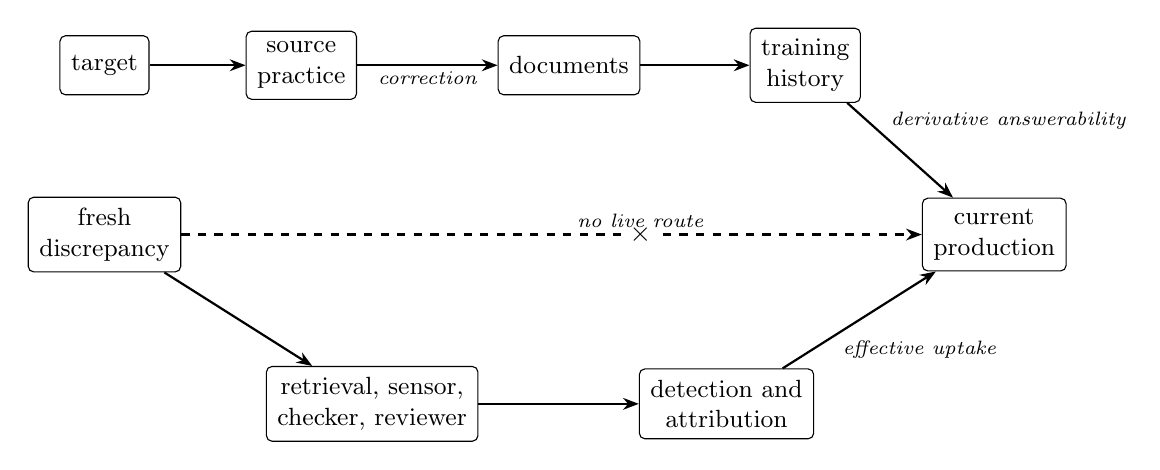
\begin{tikzpicture}[node distance=0pt]
  % historical route
  \node[ttpbox] (target) at (0,2.15)   {target};
  \node[ttpbox] (prac)   at (2.5,2.15) {source\\practice};
  \node[ttpbox] (docs)   at (5.9,2.15) {documents};
  \node[ttpbox] (train)  at (8.9,2.15) {training\\history};
  \node[ttpbox] (prod)   at (11.3,0)   {current\\production};

  \draw[ttpar] (target) -- (prac);
  \draw[ttpar] (prac) -- node[ttplab, below] {correction} (docs);
  \draw[ttpar] (docs) -- (train);
  \draw[ttpar] (train) -- node[ttplab, above right, pos=0.35]
        {\term{derivative answerability}} (prod);

  % the fresh discrepancy, with no route of its own
  \node[ttpbox] (fresh) at (0,0) {fresh\\discrepancy};
  \draw[ttpblocked] (fresh) -- node[pos=0.62, fill=white, inner sep=1.5pt] {$\times$}
        node[ttplab, above, pos=0.62] {no live route} (prod);

  % a live route, added
  \node[ttpbox] (route) at (3.4,-2.15) {retrieval, sensor,\\checker, reviewer};
  \node[ttpbox] (det)   at (7.9,-2.15) {detection and\\attribution};
  \draw[ttpar] (fresh) -- (route);
  \draw[ttpar] (route) -- (det);
  \draw[ttpar] (det) -- node[ttplab, below right, pos=0.35]
        {\term{effective uptake}} (prod);
\end{tikzpicture}
\caption{Derivative and live answerability. The historical route supplies derivative
answerability only where target-sensitive correction survives in the training
distribution. Dense causal ancestry alone supplies none to the empirical target at
issue: a propaganda corpus can leave equally persistent traces while answering instead to
audience response or institutional discipline. A discrepancy arising after the training
history is fixed has no route of its own. It reaches production only where a live route is
active in the arrangement, which is a fact about the arrangement rather than about whether
the weights can change.}\label{fig:routes}
\end{figure}

Inherited participation by itself never supplies live answerability. Once the training history is
fixed, a discrepancy arising after it has no way to reach production. Training against
verifiable rewards tests this boundary. When a model is optimized against unit
tests, a proof checker, or execution results, a discrepancy between output and an
independently specified target is detected and does alter production. All five features can
be instantiated while the verifier runs, to the extent that it's adequate to the target,
sufficiently independent of the generator, and attributable in its signal. Tests can be
incomplete, attribution coarse, and verifier errors correlated with the generator's.

The training process has then been corrected; the deployed arrangement isn't thereby
correctable. The training loop delivers corrective control only over the targets its
verifier covers and only while it runs. A model that has
learned arithmetic against a checker still can't tell you whether today's figure is right.
Verifiable rewards can strengthen derivative answerability, since the corrections they
encode were made against an independently specified target rather than against approval alone.
They don't make it live.

Operational participation supplies target access. Corrective
participation is where detectability, attribution, and effective uptake usually enter, and
only when the feedback is attributable and reaches production. A merely decorative
invocation supplies none of them through the purported route while resembling all of them.
Checking-route independence belongs to none of the modes in particular, since it depends on
where a checker came from and what it can see rather than on how it participates.

Corrective control is bounded by the union of the arrangement's live routes, and it's
bounded target by target. A user who checks a claim can supply corrective capacity for
that claim. How often users check fixes the route's exercise frequency across claims; how
often checking reduces a relevant, detected, attributable discrepancy, and how often it
intervenes harmfully, determine realized effectiveness. A routinely bypassed checking step
adds nominal capacity but little exercise. So the interesting case isn't an arrangement with
no corrective control anywhere, which is rare, but the ordinary one in which an arrangement is
asked about targets that no participant can independently check. Grounding is untouched by
that boundary. Corrective control stops at it.

Participation doesn't collapse into metaphor. Inherited
participation explains why a text-only arrangement can handle a domain whose
records are dense and stable. Operational participation explains why retrieval and tools
can matter at deployment as well as during training. Corrective participation explains why
feedback contributes corrective capacity only when it can change future behaviour in
target-improving ways tied to the relevant error.

The modes are individuated before the performance test by causal and architectural facts:
training objective, data
provenance, filtering history, runtime information flow, tool-call logs, sensor access,
update mechanisms, and the route by which feedback changes later behaviour. Performance
on held-out cases then tests whether this classification supports the declared projections.

Decorative participation is the failure mode: the language of measurement without
measurement; the language of citation without a record.

\subsection{Route-specific interventions}

The main interventions can be described in stabilizer terms. Retrieval augmentation
queries an external corpus or search system and places retrieved material into the
model's context; it adds record access when it works. Its characteristic failures are
diagnostic rather than incidental: a stale index supplies a record of the wrong time, a
chunk boundary supplies half a record, and an embedding match on wording rather than
content supplies a passage that resembles the answer. Each leaves the archival route
nominally present and materially absent, which is decorative participation arriving
through a mechanism rather than through a turn of phrase.

Tool use routes a subtask through a calculator, database, code interpreter, application
programming interface, or instrument; it adds calculation or measurement only when the
right tool is called and its
result is integrated. When execution results guide revision, tool use adds a corrective
loop as well.

Self-consistency prompting samples multiple completions or reasoning paths and privileges
convergence among them; it strengthens internal convergence. An external check requires a
route to the relevant facts whose signal isn't generated by the same convergence process.

Instruction tuning and RLHF change the model's policy through demonstrations,
preferences, benchmarks, or evaluations; they add a social or evaluative correction
route whose target depends on the feedback.\footnote{Preference signals have factual
targets. Rater approval of affirmation, deference, or confident presentation is a fact
about a population and interaction setting, and RLHF can make the resulting arrangement's behaviour
strongly answerable to that fact. The failure mode is target mismatch: the policy can
track the rater distribution accurately while its assertions are assessed against a
different, object-level target. Sycophancy is the clean case, where an arrangement accurately
tracks the wrong target.}

Multimodal input supplies image, audio, video, or sensor information; by itself, it adds
perceptual input. Calibrated measurement is a separate stabilizer.

Multimodality matters because it seems to answer
\posscite{harnad_1990_symbol_grounding_problem} sensorimotor prescription. This profile
gives a finer-grained diagnosis. His proposal joins perception to action, correction, and
use. An arrangement built around a vision-language model trained on image-caption corpora
has inherited perceptual participation through selected, framed, and captioned images. A
deployment-time image input adds operational perception. Those
routes supply perceptual input; calibrated measurement, intervention, and action-guided
correction remain separate stabilizers.

Multimodal input should improve performance unevenly. It should reduce some failures in
object classification and leave measurement- and intervention-dependent tasks fragile.
It should also leave room for object hallucination, where generated descriptions include
objects not present in the image
\citep{li_etal_2023_evaluating_object_hallucination_lvlms}. That pattern is what this
account expects when target access is strengthened and the correction routes are left
as they were.

To test this view, hold the topic, answer format, and apparent difficulty fixed, and vary
the missing stabilizer. Gains should follow the added routes. Retrieval should improve
source-backed recall more than novel measurement or action-sensitive causal judgement.
Self-consistency should improve coherence-sensitive reasoning more than claims that need
a fresh route to the facts. Multimodal input should improve perceptual classification
before it improves calibrated measurement. If gains transfer evenly across those
contrasts, that would be evidence that this profile has carved the stabilizers badly.

A deployed product may occupy several rows at once. A chat system can be
instruction-tuned, retrieval-augmented, partly tool-using, and multimodal. This profile
asks which stabilizer is live in the task being assessed.

Which profile counts as the baseline depends on the task. The text-only case gives the
cleanest pressure test: it's a limiting, task-relative position rather than a description
of a product. Arrangements built around models trained on interleaved image and text, on
code corpora, or against verifiers occupy richer positions. When retrieval, tools, or multimodal routes are idle,
inappropriate, or unintegrated, the arrangement has the text-only profile for that task.

The limiting case still inherits reports written by perceivers, explanations corrected by
teachers, institutional records, and descriptions shaped by instruments. It can
support genuine epistemic achievements while occupying a different role from a speaker or
hearer in a testimonial exchange.

Table~\ref{tab:llm-profiles} summarizes the architecture-sensitive predictions. The rows
are profiles rather than a scale from bad to good.

\begin{table}[H]
\centering
\small
\begin{tabular}{@{}>{\raggedright\arraybackslash}p{0.20\linewidth}>{\raggedright\arraybackslash}p{0.34\linewidth}>{\raggedright\arraybackslash}p{0.36\linewidth}@{}}
\toprule
Arrangement type & Principal architectural resources & Directional prediction \\
\midrule
Text-only pretrained model & Training-distribution regularities and local coherence & Strong where dense,
stable text is a good proxy; fragile for recent, obscure, perceptual, or measurement-dependent facts. \\
Instruction-tuned or RLHF model & Rater feedback, demonstrations, and benchmark evaluation & Better conversational fit and some error reduction; independently informative checking routes still have to be supplied. \\
Retrieval-augmented system & Live access to records and institutional traces & Better on updated or source-backed recall; remaining fragility where the missing route is experiment, perception, or intervention. \\
Tool-using or coding system & Calculators, databases, code execution, instruments, or application programming interfaces & Better where the right tool is called and interpreted; strongest when runtime or test results guide revision; new failures from tool choice, stale data, and test-as-proxy effects. \\
Multimodal system & Perceptual input in image, audio, video, or sensor form & Better for some perceptually anchored tasks; calibrated measurement and practical correction remain separate stabilizers. \\
Action-guided or expert-reviewed system & Practical feedback, review, and downstream failure pressure & Stronger corrective capacity where feedback is timely and domain-competent; weaker where review is sparse or proxy-based. \\
\bottomrule
\end{tabular}
\caption{Architecture-sensitive profile predictions.}
\label{tab:llm-profiles}
\end{table}

\subsection{Inherited structure and missing anchors}

Documentary inheritance cuts both ways. Human text is saturated with world-directed
practice. It contains the residue of people looking, measuring, arguing, repairing,
citing, and correcting one another. The deployed arrangement usually remains outside those
practices when it produces a fresh answer. It draws on their products with attenuated access to
their present checks.

Text-only training can still produce more structure than a bare \mention{textual
residue} slogan suggests. The generative pretrained transformer model Othello-GPT is an
important pressure case: a sequence model trained to predict legal moves in a board game
developed an internal representation of board state, and interventions on that
representation affected its outputs \citep{li_etal_2023_emergent_world_representations}.
Such cases fit this account where the target structure is densely and systematically
encoded in the sequence stream. They show that inherited
participation can be strong when the relevant world is small, rule-governed, and
recoverable from the training signal.

Othello is a thin base for a claim this size. It's finite, fully observable, and its legal moves are a deterministic function
of a state the move sequence determines, so the training signal contains the world
entirely. The result is striking for that reason and unrepresentative for the same one.
Nothing follows about domains where the state isn't recoverable from the record, which is
the class this argument concerns. What the example establishes here is
narrower, that inherited participation isn't limited to surface statistics when the world
is small enough to fit in the stream.

Limits matter. Internal world-model evidence should be strongest where the relevant
state variables are encoded in the sequence and the loss function penalizes violations
of their structure. It should weaken when success depends on variables absent from the
sequence, live measurement, changing local conditions, or intervention in the target
system. Successful transfer across those boundaries would count against this diagnosis.

Alongside documentary inheritance, coherence is another stabilizer in which these
arrangements participate strongly. Training and decoding reward genre fit,
local well-formedness, smooth inference, and continuation from context. Those
pressures explain why these models can display impressive formal linguistic competence,
in the sense separated from functional world use by \textcite{mahowald2024}. They also
explain the vulnerability. Coherence can improve the shape of an answer and add no
independently informative route by which the relevant facts constrain it.

In the baseline profile, perception, measurement, intervention, and practical correction
enter weakly through text produced by others. A model can generate a
plausible lab result, legal summary, local observation, or bibliographic claim because
similar text exists. Present production remains unconstrained by an experiment, court
record, observation, or catalogue entry.

Textual inheritance is reliably distributional and only contingently archival. Training
can and does preserve particular strings, names, and sources, so this claim isn't that
token-bound information never survives. It's that nothing preserves it under a general
relation of record identity, provenance, and current checkability. Training
preserves redundantly represented patterns more reliably than material carried by a single
passage. A text-only model can encode statistical regularities in testimonial practice.
The resulting arrangement can handle a domain whose records are dense and stable while
fabricating the verbatim anchors (quotations, identifiers, author lists) on which the
practice's correction routines depend. The same distinction predicts that these failures should be especially
retrieval-sensitive: retrieval adds the archival route that distributional inheritance
lacks.

Hallucination plays a more specific role here. The LLM literature treats it as heterogeneous
\citep{huang_etal_2025_survey_hallucination_llms}. This profile makes a narrower claim:
text-only arrangements should be especially vulnerable to fluent, coherent, genre-appropriate
outputs that fail when the task requires a fresh or independently informative route to the facts.
Those failures should be common for obscure sources, recent events, local observations,
novel measurements, fine-grained quantities, and action-sensitive causal claims. They
should be less common where dense, stable, redundant text is already a good proxy.

Frankfurtian accounts of bullshit \citep{frankfurt_1986_on_bullshit} diagnose LLM output
differently. \textcite{hicks_humphries_slater_2024_chatgpt_bullshit} apply that diagnosis
to ChatGPT-style systems, arguing that their outputs are produced with indifference to
truth. On the Frankfurtian diagnosis, the system doesn't care where the facts are; on this
diagnosis, the relevant facts have no route into production or correction. That
missing route yields comparative predictions across retrieval, tools, multimodality, and
action-guided feedback. This diagnosis asks for a route, not a better attitude.

Mitigation results should be read through the same distinction. Retrieval can reduce
hallucination in conversation \citep{shuster2021retrieval}; that's evidence about record
access. Perception, experiment, and intervention require further routes. Tool use and
multimodality make parallel changes. They add operational routes where the tool, sensor,
or modality is live in the task; otherwise the new vocabulary of tools or
perception can remain decorative.

Action-guided arrangements can provide the table's broadest corrective upgrade when the
feedback is timely, attributable, and tied to the relevant failure. Coding is the clean
artificial case. An arrangement that runs generated code, observes a compiler error, traceback,
failing test, or successful execution, and revises against that result has a tighter
corrective route than one rewarded for plausible-looking code. A robot that breaks a
glass, misses a target, or fails a laboratory protocol can receive similar correction
unavailable to a text-only arrangement. A deployed chatbot that receives delayed approval,
engagement metrics, or sparse user edits has a thinner corrective route. The label
\mention{feedback} hides that difference unless the stabilizer is specified.

\subsection{What the correction routes correct}

Instruction tuning, RLHF, benchmark evaluation, red-teaming, and expert review function as
correction routes, and they should be classified by what they correct. Their immediate
targets often include helpfulness, harmlessness, preference satisfaction, conversational
fit, and benchmark success. Those constraints can reduce some errors and can also reward
answer-shaped behaviour when users or raters prefer confidence, agreement, or plausible
explanation.

Post-training isn't one thing, and this profile begins by splitting two cases. Where the
reward comes from a rater's approval, the immediate optimization target is that approval.
Where it comes from a unit test, a proof checker, or an executed result, the correction is
answerable to an independently specified criterion, to the extent that the checker is
adequate to the target.
Both are called post-training and they build different profiles. Treating checker-based
reward as mere rater approval understates what it supplies; treating rater approval as
truth-directed feedback overstates it. The relevant question is never how much post-training an arrangement
received but which targets its rewards were computed against.

Work on sycophancy shows the risk of treating feedback based on human preference
judgements as truth-directed on its own \citep{shapira2026rlhf}. In this profile's terms,
these processes strengthen some social and evaluative constraints while leaving target
contact through perception, measurement, and intervention indirect or absent.

Accounts of fine-tuning disagree because they address different explananda.
\textcite{grindrod_2024_large_language_models_linguistic_intentionality} treats it as a
relatively marginal procedure that can't be what makes the difference between
intentionality and its absence, since models produce apparently meaningful text without
it. \textcite{ruyant_2026_what_do_llms_represent} treats it as constitutive of what the
system represents, because the norms of appropriateness a model is tuned toward are what
fix its target.

The claims concern different explananda. Fine-tuning can be constitutive of appropriateness
for a purpose, Ruyant's explanandum, because norm setters fix that purpose. It can remain
marginal to whether outputs are meaningful in Grindrod's sense. Neither verdict settles
target-directed correction. Rater approval supplies that only when the judgement is
informed by a target-sensitive route: fact-checking against records, tool results, or action outcomes
rather than approval alone. Treating all three questions as one quantity called grounding
makes the disagreement look unresolvable.

\subsection{What grounding leaves open}

\textcite{coelho_mollo_milliere_2026_vector_grounding_problem} press the strongest
neighbouring challenge. They distinguish kinds of grounding and argue that some LLM
states can satisfy causal-historical or teleosemantic conditions for referential
grounding. Their conclusion isn't in
dispute. This account's explanandum is broader than referential grounding.

Work on neural word embeddings pushes in a similar direction: learned representations
may have genuine, though limited, contents fixed by the functions they serve inside the
system \citep{mallory_2026_teleosemantics_word_embeddings}.
Teleosemantic pressure of this kind fits the baseline text-only case. The reply concedes content and
asks which stabilizers that content participates in.

Training text carries correction procedures,
defeaters, and records, and a model can learn to reproduce some of them. What
inheritance alone doesn't deliver is a live route by which a fresh discrepancy reaches
production and changes it.

Referential grounding covers one dimension of world-connection. Truth-tracking answerability
depends on a wider profile of stabilizers, including correction, measurement,
intervention, perception, and practical feedback. An LLM state might be referentially
grounded in their sense even as the deployed arrangement has a fragile truth-tracking profile
for tasks requiring independent checking.

\textcite{mandelkern_linzen_2024_do_language_models_words_refer} make the gap vivid. They
close with Izzy, isolated from
birth in a sensory-deprivation chamber and reaching the world only through a text screen,
and they argue that externalism dissolves the puzzle about how his words
refer. Izzy's
answerability is nonetheless confined to the testimonial and inferential routes his screen
supplies, with perception, measurement, and intervention absent. Secure reference
alongside a radically restricted profile is the dissociation at issue.

Pepp presses the harder version \citep{pepp_2025_reference_without_intentions_llms}. She
suggests that such systems may contact objects
through their exchanges with users, coming into contact with whatever shaped a user's
input. The participation distinction
splits that case. A live image-input route supplies operational perception, and this profile
says so. Contact with the objects that shaped a user's text is inherited: the perceiving
was done by someone else, and nothing in the exchange reports back when the user was
wrong.

Bender and Koller's octopus and Mandelkern and Linzen's Izzy are used to pull in opposite
directions on reference. Their shared limit is architectural. In each case, linguistic
traffic is the principal route, so a discrepancy that never enters that traffic can't
alter present production. What isn't on the wire can't correct what is.

\subsection{Corrective control in deployment}\label{ssec:deployment}

A deployed case shows what adding a checker takes. \textcite{anthropic2026automode}
describes a coding agent that routes each proposed action through a classifier that blocks
operations it judges irreversible, destructive, or aimed outside the working environment.
The case concerns safety control rather than factual truth
directly. Its role here is to isolate the architecture by which a separate discrepancy
signal becomes behaviourally effective.

When its policy judgement is correct, the separate classifier can supply detection and
effective gating where the acting model registers nothing itself. It thereby supplies
detectability and effective uptake through a second party rather than through introspection.

Separation alone doesn't secure checking-route independence. An external checker can
reproduce the generator's errors, while the same model given independently sourced
environmental information may not. Relevant dimensions include development provenance,
the environmental information available to the checker, objectives, and conditional error
structure. The reported hardening gave the classifier more environmental information,
including repository visibility and git state. Whether that change decorrelated its errors
wasn't measured, and lineage alone wouldn't settle the question. Measuring it requires
conditional error rates for checker and generator on a shared held-out set.

The approval step's contribution also depends on its use. Users reject 3\% of individual
permission requests against 39\% of plans put to them for approval. The permission route
isn't decorative outright, since a rejection can alter the action. But the 3\% figure
records rejection frequency, not realized corrective effectiveness; without audited rates
of genuinely unsafe proposals and false blocks, effectiveness is unidentified.\footnote{Same users and product, two approval arrangements, which is consistent
with route-specific non-exercise though it doesn't isolate the route from interface
burden, action granularity, or perceived stakes. A controlled study points the same
way, with human testers catching 13.6\% of planted dangerous commands against the
classifier's 89\%, though its participants worked in a purpose-built environment and knew
they were being evaluated \citep{anthropic2026automode}. Both figures are a vendor's
self-report about its own product and haven't been independently audited. In this paper about
independent checking, the evidence comes through a reporting arrangement with a profile of
its own. The figures are used here
to illustrate the availability and exercise gap, not to measure it.}

\subsection{Empirical transfer}\label{ssec:transfer}

Route-specific transfer gives the strongest test. Improvements in one route should remain
limited where a task depends on a different stabilizer. If reliable perception,
measurement, retrieval, tool use, expert correction, or action feedback fails to alter
the expected contrast in the direction just specified, this profile has misdescribed the
mechanisms. If text-only arrangements remain mainly dependent on inherited textual
accommodation and local coherence, the same vulnerability should persist even as fluency
improves.

A clinical test makes this concrete.\footnote{The design parallels validity
argumentation in measurement: inferences from performance are licensed relative to a
purpose and tested by varying method while holding the target construct fixed
\citep{messick_1989_validity,kane2013validating}.} One item set asks for recommendations
recoverable from guidelines or institutional records. A paired set uses the same disease
area and answer format and requires a patient-specific lab value, observed sign, dose
calculation, or intervention-sensitive causal judgement. This profile
predicts a retrieval gain on the record-recoverable set and little transfer to the
patient-specific set unless the needed measurement or tool route is supplied. Retrieval alone producing the same gain on
both sets would count against the carving.

Matching the sets on difficulty cues won't do. An
intervention that supplies a missing lab value also makes the item easier, so a
difficulty explanation and a route explanation both predict a gain, and a cue-matched
design can't separate them. Equating on measured baseline accuracy weakens the simplest
version of the difficulty story without eliminating it: two sets can share a baseline mean
and differ in discrimination, ceiling structure, response variance, latent subskills, or
treatment-effect heterogeneity. Matching on noisy estimates also invites regression to the
mean. Treat baseline performance as a covariate and a design diagnostic, not as proof that
difficulty has been removed.

The primary design is crossed rather than matched. Build item families in
which the relevant route can be supplied or withheld within closely related items, then
cross route availability against task requirement. Estimate the interaction in a
hierarchical model with varying effects for items, domains, prompt templates, and systems.
Declare in advance the smallest interaction that would matter, report the interval rather
than a verdict, and run reasonable alternatives for item matching, scoring, and exclusion
instead of resting on one sample.

For the retrieval case, the source feature is whether a live retrieval route over a fixed corpus is
available. The outcome is substantive correctness of the recommendation, scored blind, which
applies to both halves of the item set. Whether verbatim anchors resolve is a secondary
outcome and applies only within the record-dependent half. Making anchor resolution primary
would manufacture the interaction, since patient-specific items have no corpus anchors to
resolve and would fail by construction rather than by hypothesis.

The bearers are two named chat arrangements that differ only in whether retrieval is
available, with the prompt template held constant. The estimate is conditional on that pair
and settles nothing about variation across models or deployment setups. The population is
a clinical item set split into record-recoverable and
patient-specific halves, classified from the item text by raters who see no system output,
and frozen before the first run.

The prediction is an interaction, with the retrieval gain on record-recoverable items exceeding
the gain on patient-specific items by at least ten percentage points. Ten is a worked value
rather than a derived one. Fixing it properly needs a decision basis the carving doesn't
supply: the cost of a wrong recommendation, the cost of retrieval latency, and what a
deployment would do differently at nine points rather than eleven. Stating it anyway is what
makes the prediction refusable.

Interpretation then runs against ten rather than against zero. An interval concentrated
above ten supports this claim. An interval concentrated near zero, or on the wrong side,
counts against it. An interval running from below zero to well above ten reports an
uninformative experiment rather than evidence either way, which is the case a bare
significance rule would misread as a refutation. The decision threshold isn't revised once
the effect is visible. If it has to be, that's the result.

One interaction is weaker than two. Retrieval should help the record-dependent items, and
a measurement tool should help the measurement-dependent ones, so
crossing both interventions against both task types tests a double dissociation. That
tests whether the proposed routes track selective transfer, but the interaction isn't
unique to this profile. A relevance-sensitive information account can predict the same
qualitative crossing by treating records and measurements as different task-specific
information.

Coverage has three readings. \term{Content coverage} concerns answer-relevant content
currently accessible in a prompt, retrieved passage, database response, sensor output, or
other input. Content coverage is a restricted empirical comparator: two arrangements can
have the same content coverage while differing in what they do with it.

\term{Conditional coverage} concerns what one route adds given what the other routes have
supplied. It can represent the greater value of a checker whose errors don't reproduce the
generator's. \term{Effective coverage} includes whatever information can influence the
final output given the architecture, provenance, checking relations, and uptake policy. It
summarizes the usable information supplied by the whole arrangement without decomposing how
it became usable.

The clearest competing account uses content coverage. Conditional coverage remains an
empirical comparator when its measure is fixed in advance, but it already incorporates
checking-route independence and joint error structure. Effective coverage includes nearly
the whole profile. Used without fixed application conditions, it can absorb any result by
counting each helpful route as an increase in coverage. It then functions as a reduced-form
summary of the profile rather than a rival mechanism. Effective coverage may serve coarse
retrospective prediction while this profile serves intervention, audit, and transfer.
Nothing here requires one uniquely correct description for both purposes.

This yields an identification limit. For any mapping from profile features and environments
to performance, an unrestricted coverage variable can be defined to reproduce that mapping.
Behavioural results alone can't identify which architecture produced the usable information.
Lineage, information flow, conditional error structure, and update routes supply the
additional evidence. The empirical comparison needs fixed application conditions specified
before the outcomes are observed.

The burden falls on this profile's factorization. Its five features are characterized from
architecture and history before performance is measured. Compare a prespecified
content-coverage model with the profile model on held-out combinations of routes, tasks,
and perturbations without changing what their variables mean. This profile earns its keep
if the decomposition improves prediction, predictive calibration, transport, diagnosis, or
intervention. It loses if content coverage predicts the contrasts equally well, or if the
five features add no transportable value. Calibration history earns a place only where it
helps characterize those features or their stability under perturbation.

The decomposition also has practical content. It should help choose among retrieval,
measurement, independent checking, and enforced uptake before their returns are observed.

A sharper test targets checking-route independence. Compare two checkers: one from the
generator's lineage, the other trained and calibrated on separate data and feedback. Match their runtime evidence,
standalone accuracy, confidence, latency, response format, and revision policy as closely
as possible. Measure
detection and correction conditional on generator error, especially under perturbations
expected to produce common-mode failure.

This profile predicts an advantage for the checker with lower conditional error overlap.
For this contrast, calibration history matters only insofar as it predicts that overlap; if admissible
perturbations produce no difference, this profile has no reason to privilege one history.
A content-coverage account predicts no advantage once access and marginal competence are
matched. A conditional-coverage account can predict one by representing the joint error
structure, but that account has then incorporated the relation that checking-route
independence names.

The temporal manipulation serves a different purpose. Give two arrangements the same target
information at the outset, one holding a frozen pasted record and one holding a live route
to its source. In the update arm, correct the source record and ask a follow-up whose answer
turns on the correction. In the control arm, leave the record unchanged. The live route
should track the update in the first arm and match the frozen copy in the second.

A dynamic coverage account predicts the same pattern because information available at follow-up
differs. The manipulation operationalizes live answerability; it doesn't adjudicate between
the two descriptions.

Figure~\ref{fig:design} sets the arms out.

\begin{figure}[H]
\centering
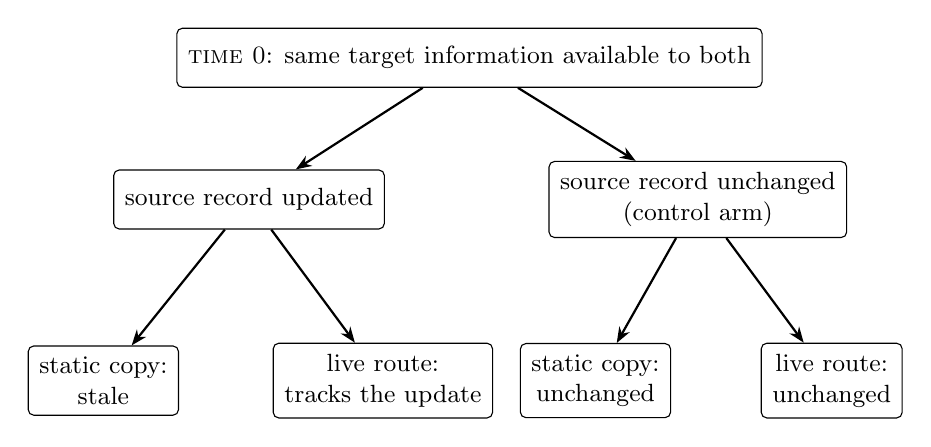
\begin{tikzpicture}
  \node[ttpbox] (t0) at (5,2.5) {\textsc{time 0}: same target information available to both};

  \node[ttpbox] (upd) at (2.2,0.7) {source record updated};
  \node[ttpbox] (ctl) at (7.9,0.7) {source record unchanged\\(control arm)};

  \node[ttpbox] (u1) at (0.35,-1.6) {static copy:\\stale};
  \node[ttpbox] (u2) at (3.9,-1.6)  {live route:\\tracks the update};
  \node[ttpbox] (c1) at (6.6,-1.6)  {static copy:\\unchanged};
  \node[ttpbox] (c2) at (9.6,-1.6)  {live route:\\unchanged};

  \draw[ttpar] (t0) -- (upd);
  \draw[ttpar] (t0) -- (ctl);
  \draw[ttpar] (upd) -- (u1);
  \draw[ttpar] (upd) -- (u2);
  \draw[ttpar] (ctl) -- (c1);
  \draw[ttpar] (ctl) -- (c2);
\end{tikzpicture}
\caption{A temporal test of live answerability. At time 0, the same target information is
available to both arrangements. In the update arm, the source record is corrected: the
static copy remains stale, while the live route can transmit the correction. In the
control arm, neither should change. The contrast isolates updateability from initial
content equivalence. It's compatible with a dynamic coverage account that treats current
access as part of information availability. No outcome magnitudes are implied.}\label{fig:design}
\end{figure}

Failure of the declared route-specific interactions or update effects, after confirming
that the relevant route was invoked and its output reached production in time to affect the
answer, would defeat this carving. The deployment case changed environmental access without
measuring error correlation, so it bears on one feature rather than testing the
factorization.

Observing that every grounded arrangement in some sample also corrects well wouldn't show
that grounding entails corrective control: both might depend on a third architectural
feature, or every arrangement sampled might satisfy more than the grounding conditions require.
Non-entailment isn't refuted by co-occurrence.

\section{Conclusion}\label{sec:conclusion}

The octopus and Izzy support opposing verdicts on reference, but this paper's question
survives either one. Representations can have content, reference, and correctness
conditions while the output-producing arrangement lacks live, sufficiently independent
routes from detected discrepancies to altered production. Grounding doesn't entail
corrective control.

Language-model arrangements make the dissociation visible at scale. Their models inherit
dense textual residues of testimony and coherence. Those residues supply derivative
answerability where source practices have already made target-sensitive corrections, while
the arrangements may participate weakly in routes that detect a fresh error and carry it
back into production. Identifying which
routes an arrangement has, at what strength, and for which targets shows when the gap has
been closed rather than merely narrowed. Rich internal structure can arise where
the target domain is densely encoded in the sequence stream without supplying those live
routes elsewhere.

A thin truth predicate can coexist with thick truth-tracking practices. Recurrence of a
profile supports a stability claim; where specified dependencies sustain that recurrence,
the profile may be effectively maintained. Corrective control adds live capacities for
detection and repair. None of that architecture need be built into truth itself.

The older epistemologies keep their subject matter. Each can represent relations among
the processes it describes, and reliabilists and social epistemologists routinely do. The
default basis for projection here is an arrangement's calibration history among sources
rather than a single process assessed against that background. In ordinary cases the routes run together;
language models make their separation visible.

Comparison rather than classification follows. Effective coverage can summarize whether an
arrangement had usable information, but it doesn't by itself say which intervention to
choose or where a gain should transfer.

Retrieval, multimodal input, tool use, expert review, experimental embedding, and
action-guided feedback alter an arrangement's stabilizer profile. The question is which route they add,
whether that route is live in the task being assessed, and where improvement should
transfer. The route-by-task interactions aren't unique to this profile. Its stronger burden
is to predict held-out combinations of interventions and tasks from a fixed factorization
better than a prespecified content-coverage model. An arrangement can improve along one dimension
and remain fragile along another. Participation is classified by causal and architectural facts
before performance is checked, and the predicted contrasts can fail.

The pressure case generalizes. Truth-tracking extends beyond linguistic competence,
internal coherence, and statistical sensitivity to past assertion. It depends on a wider
ecology of correction. What matters is which routes an arrangement participates in, which
it borrows, which it lacks, and where those absences should matter.

\section*{Acknowledgements}
I thank Geoff for comments on coherence theory and the history of \mention{true}.

\clearpage
\printbibliography

\end{document}
